\chapter{Compositional Surrogate}\label{sec:concept}

    \epigraph{``All models are wrong but some are useful``}{\textit{– George Box}}

    This chapter introduces a general idea which overcomes the limitations of model-based optimization discussed.

    As mentioned previously in section ~\ref{sec:background}, fixed components can make the optimization process ineffective. That is why flexibility and variability must be introduced for each optimization step. Our concept focuses on the combination of surrogate models to effectively extrapolation required problems.


    % --------------------------------------------------------------------------------------------
    % ------------------------------------------------     RG1: Models combinations     
    % --------------------------------------------------------------------------------------------

    \section{Combinations of surrogate models}

        Let us address the main issue we have observed in multi-objective optimization. The issue is that the solution techniques and parametric selections are usually problem-specific. In addition to that, most surrogate model implementations are static which imposes limitations on existing solutions. We tackle this challenge by improving model variability \emph{in} a surrogate model (compositional surrogate) and model extensibility \emph{with} surrogate hypotheses (surrogate portfolio). Also, we should address an additional question of solution scalability, which is related to the compositional surrogate model. There are some tasks that could require new algorithmic approaches when we add more parameters to them. Therefore, there exists a demand for scalable solutions. We discuss our approach to problems described i+n the next sections.

        % ------------------------------------------------     Compositional model      
        \subsection{Compositional Surrogate Model [RQ1]}
            The concept of the compositional surrogate is the combination of multiple simple models to approximate several independent objectives at the same time. In this model, composite and conventional surrogates have a unified interface that permits us to implement a \emph{composite design pattern}\cite{bookGOF}. This design pattern then allows us to operate uniformly with the individual and multi-objective surrogates. 

            Additionally, a significant advantage of compositional surrogates is a possibility to extend single-objective parameter tuning to multi-objective optimization. This possibility provides the opportunity to reuse single-criterion models for multi-criteria optimization and dynamically reconstruct problem representation from mixed parts.
            We define \emph{compositional models} as models that combine \emph{various} sub surrogate models for each optimization objective. The \emph{surrogate hypothesis} refinement is also used to emphasize that the surrogate model can completely describe all criteria from the objective space.

            The compositional surrogate has multiple opportunities for variability that outperform static models in the face of real black-box problems. For example, choosing a specific set of models is a representation of knowledge about the subject area. If expectations during optimization are not met, the compositional model can be partially updated, which saves time. In contrast, a static model would need to be completely replaced. Such changes might be demanded by newly obtained results or the increased dimensionality of optimization space.

            % ------------------------------------------------     Scalability     
            \subsubsection{Scalability}
            The ability to scale the optimization solution can be considered an adaptation to an unknown problem. Solution scalability is the ability to solve problems with a high number of dimensions in parameters and objectives spaces.

            Multiple works\cite{KrallMD15, SpringenbergKFH16} have practically demonstrated that scalability is a problem for surrogate models and optimization algorithms. As an illustration, popular surrogate models such as Gaussian process regression (Kriging) \cite{JonesSW98} struggle with high dimensional samples but provide excellent results in smaller dimensions. Therefore, another advantage of the composite surrogate model is evident; it provides variability for the extrapolation of scalable search space.

            % % -------------------------     Categorical parameters      
            % \subsubsection{Categorical parameters} 
            %     Multi-objectivity and categorical parameters are essential for real parameter tuning. On the one hand, most related works used native models that support simulation with categorical features because it is interpretative and intuitive \cite{HutterHL11, nardi2019practical}. On the other hand, the feature-encoding methods are used to turn the categorical parameter into numbers for the generic model class. Coding features for a surrogate model can transform those in a meaningful form, that a model can use to perform calculations. Based on this samples interpretation, the model might extrapolate all points in the parameter space. Several types of encoders can be used to transform any mixed parameter types into a digital representative form.
            
        
        % ------------------------------------------------     Portfolio      
        \subsection{Surrogate model portfolio [RQ2]}
            In addition to the dynamic variability in the compositional surrogate, we combine several surrogate hypotheses in a surrogate portfolio to dynamically choose one that is best suited to the specific problem. The unified interface and the ability to integrate models into a composite architecture make it possible to uniquely select and combine composite models side by side with static multi-objective models.

            Without information about a given problem, it is difficult to say which surrogate hypothesis would be better. Therefore, the model should be selected during optimization based on its usefulness (validity). The validation process involves checking how well the model extrapolates unknown data. For such validation evidence, a small portion of samples should be sacrificed. This process of data sacrifice give us two separate data sets: one for model building and another for its testing. The test score obtained from the test set is used to evaluate the model's accuracy and, accordingly, the quality of the possible corresponding solutions.
            The validation process allows us to evaluate surrogate models based on how they summarize an unknown problem.
            
            For an optimization algorithm, a portfolio can be considered either as a single model or as a collection of models. This property allows us to determine which optimization algorithms are applied to which surrogate models and how to combine such solutions. Such dynamic variability makes the multi-criteria optimization process also scalable and flexible.

            Besides, the surrogate portfolio does not limit to use the latest state-of-the-art optimization algorithms and surrogate models together.

    % --------------------------------------------------------------------------------------------
    % ------------------------------------------------     RG2: Sampling plan     
    \section{Sampling plan [RQ3]}
        After surveying the aforementioned related works, we learned that only BRISE use dynamic sampling plan while other approaches use a static sampling plan that determines an optimal number of initial samples using an outside oracle. On the contrary, BRISE is applied dynamic but still domain-dependant sampling plan. Although in most cases, we cannot receive any guidance on an unknown problem. 
        Thus, we need a dynamic sampling plan which adapts to a specific use-case.

        To obtain the adaptive sampling size we need to bind the sampling design to a validation process for the surrogate model. An optimization process is guided by sampling design when none of the surrogate models are valid (Figure \ref{fig:concept_sampling}). Validity means that the surrogate approximation can be useful for efficient global optimization.
        % ==== Sampling plan
        \begin{figure}[h]
            \centering
            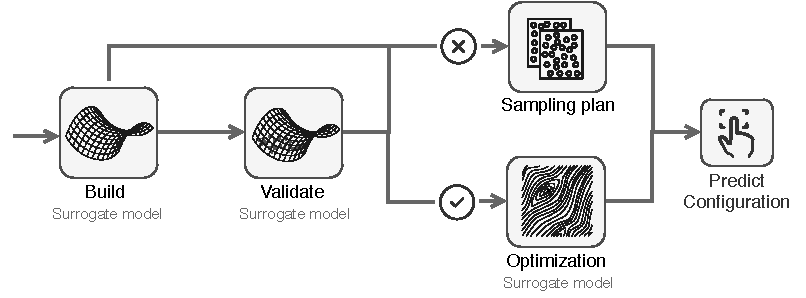
\includegraphics[width=\textwidth]{content/images/dinamic_sampling_plan}
            \caption[Non-dominated points]{Concept of a sampling plan dependency and model validation. A sampling plan is used if there is no valid model that can be useful for optimization purpose.} 
            \label{fig:concept_sampling} 
        \end{figure}      

        % -------------------------     Surrogate Validation      
        \subsection{Surrogate Validation}
        In the context of sequential model-based optimization, a common mistake is studying the accuracy of the evaluation of the global search space instead of the search space region of interest. That is why basing the evaluation of surrogate validity only on the coefficient of determination(R2) is incorrect \cite{nardi2019practical}. The global accuracy metric can be used as a threshold value above which the model becomes invalid even with additional estimations.

        It is necessary to sacrifice a small portion of samples to check the surrogate model's quality. Based on validation results, we can discard inadequate models and consider the solutions from valid models only. If none of the models are valid, the best decision is to now make a prediction from the sampling plan. This decision is repeated until a valid surrogate model is obtained.

        Validation should show how well the model extrapolates the available experiments (variance) and how well it can evaluate the data that is not seen (bias). The central concept in surrogate validation lies in the adaptation of the best machine-learning approaches for the evaluation of a model's performance. 

        We select surrogate models based on accuracy in the test set, but the selection may not be correct if only one test set is taken into account. Increasing surrogate complexity can lead to obtaining wrong conclusions in a later stage of optimization (Figure \ref{fig:cv_overfitting}). This property cannot be neglected in evaluating a surrogate's validity. 


        % ==== train\valid\test
        \begin{figure}[h]
            \centering
            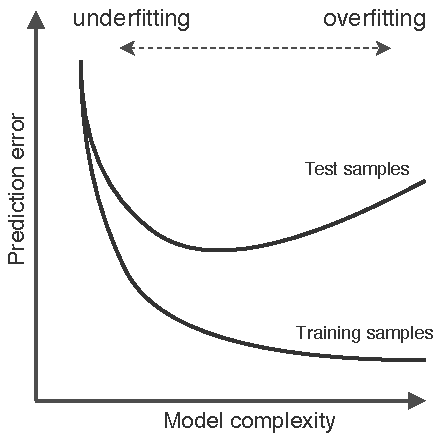
\includegraphics[width=5cm]{content/images/utility/cv_2x_test}
            \caption[surrogate validation: overfitting on the training set]{With rising model complexity overfitting on the training set becomes more likely \cite{HastieFT01, TobiasCV}.} 
            \label{fig:cv_overfitting}   
        \end{figure}

        
        It is necessary to perform the validation in a few phases with separate test sets. The validation process requires two separate test sets: the first one to select surrogate models and the second one to test those selected models. In addition to those two test sets there is a third set for building surrogate models. We obtain those sets by dividing all available samples.
        
        
        Partitioning the available samples into three sets drastically reduces the number of points that can be used for building the model. A small number of build samples could lead to inadequacy of the model. Also,results can depend on the selective random decision for sample splitting. 
        
        However, partitioning the available samples into three sets, are drastically reduce the number of points which can be used for learning the model. Moreover, results can depend on a selective random decision for the samples splitting. The solution is might be cross-validation(CV, Figure \ref{fig:cv}). This is a procedure that avoids a separate validation set and divides test samples to \textit{k} equal folds. Set of folds are used to train model and in \textit{k} rounds, a new fold selected as a test set. The performance measured by cross-validation is the averaged over the values computed in the loop. This approach can be computationally expensive but requires fewer samples. 

        % ==== train\valid\test
        \begin{figure}[h]
            \centering
            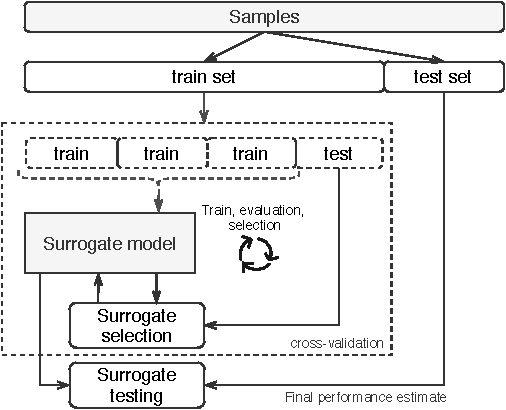
\includegraphics[width=10cm]{content/images/cv}
            \caption[Cross-validation: exploration vs exploitation]{Surrogate models validation. Cross-validation loop performs model selection based on global accuracy. Acceptable models are tested with a focus on optimization region. } 
            \label{fig:cv}   
        \end{figure}
    

        To summarize, the model validation is performed in two stages:
        \begin{enumerate}
            \item \textbf{Cross-validation.} We check overall accuracy of the surrogate model extrapolation. Also, we discard models that do not achieve the necessary threshold.
            \item \textbf{Surrogate testing.} We demonstrate the accuracy of the selected models and the corresponding assessment of possible solutions.
        \end{enumerate}
        
        We decide which surrogate models to choose based on the information from all stages. If the model does not achieve a sufficient threshold, it is rejected as not valid. If there is no valid model, the assumption about the next configuration is accepted from the sampling plan (Figure \ref{fig:concept_sampling}).


    % --------------------------------------------------------------------------------------------
    % -----------------------------------------------------       Discussion      ----------------
    \section{Discussion}
        Toward answering our research questions, we propose the dynamic combination of surrogate models and a dynamic sampling plan based on surrogate validation.
        \begin{itemize}
            \item \textbf{RQ1:} For the dynamic combination of several surrogate models, it is necessary to implement a surrogate compositional model. This design allows uniform handling of individual and compositional surrogate models.
            \item \textbf{RQ2:} The combination of surrogate models in the portfolio is realized through the compositional model and stepwise validation.
            \item \textbf{RQ3:} The sampling plan is chosen to explore new random points when there is no valid model. This relation means that the sampling plan directly depends on whether we have a surrogate model that is capable of describing the optimization problem.
        \end{itemize}
         
        As a result, we extend the idea of classic \gls{smbo} using dynamic model selection and stepwise validation to obtain a multi-objective solution on various problem landscapes. 
